\section{Sensitivity Analysis}

As detailed in the previous section we have based our processor model core properties on the Nehalem~\cite{Thomadakis2011} architecture.
In order to gain a better understanding of this model, we selected a total of five different properties we believe to have an impact on the performance of simulated benchmarks.
We then varied those five properties, one at the time keeping the others constant, and then ran all our benchmarks on the resulting system. 
For each run, we calculate the average speed-up of the benchmarks compared to the base configuration.
What we want to accomplish with this experiment is to gain an understanding of the model's sensitivity to property changes. 
If we observe a significant performance improvement when changing one of the properties, it might be an indication of a bottleneck that could skew our results.

\begin{figure}[ht]
        \centering
        \begin{subfigure}[b]{0.5\textwidth}
                \includegraphics[width=\textwidth]{figures/processor_model/ol}
                \label{fig:processor_model:sensitivity:ol}
        \end{subfigure}%
        \begin{subfigure}[b]{0.5\textwidth}
                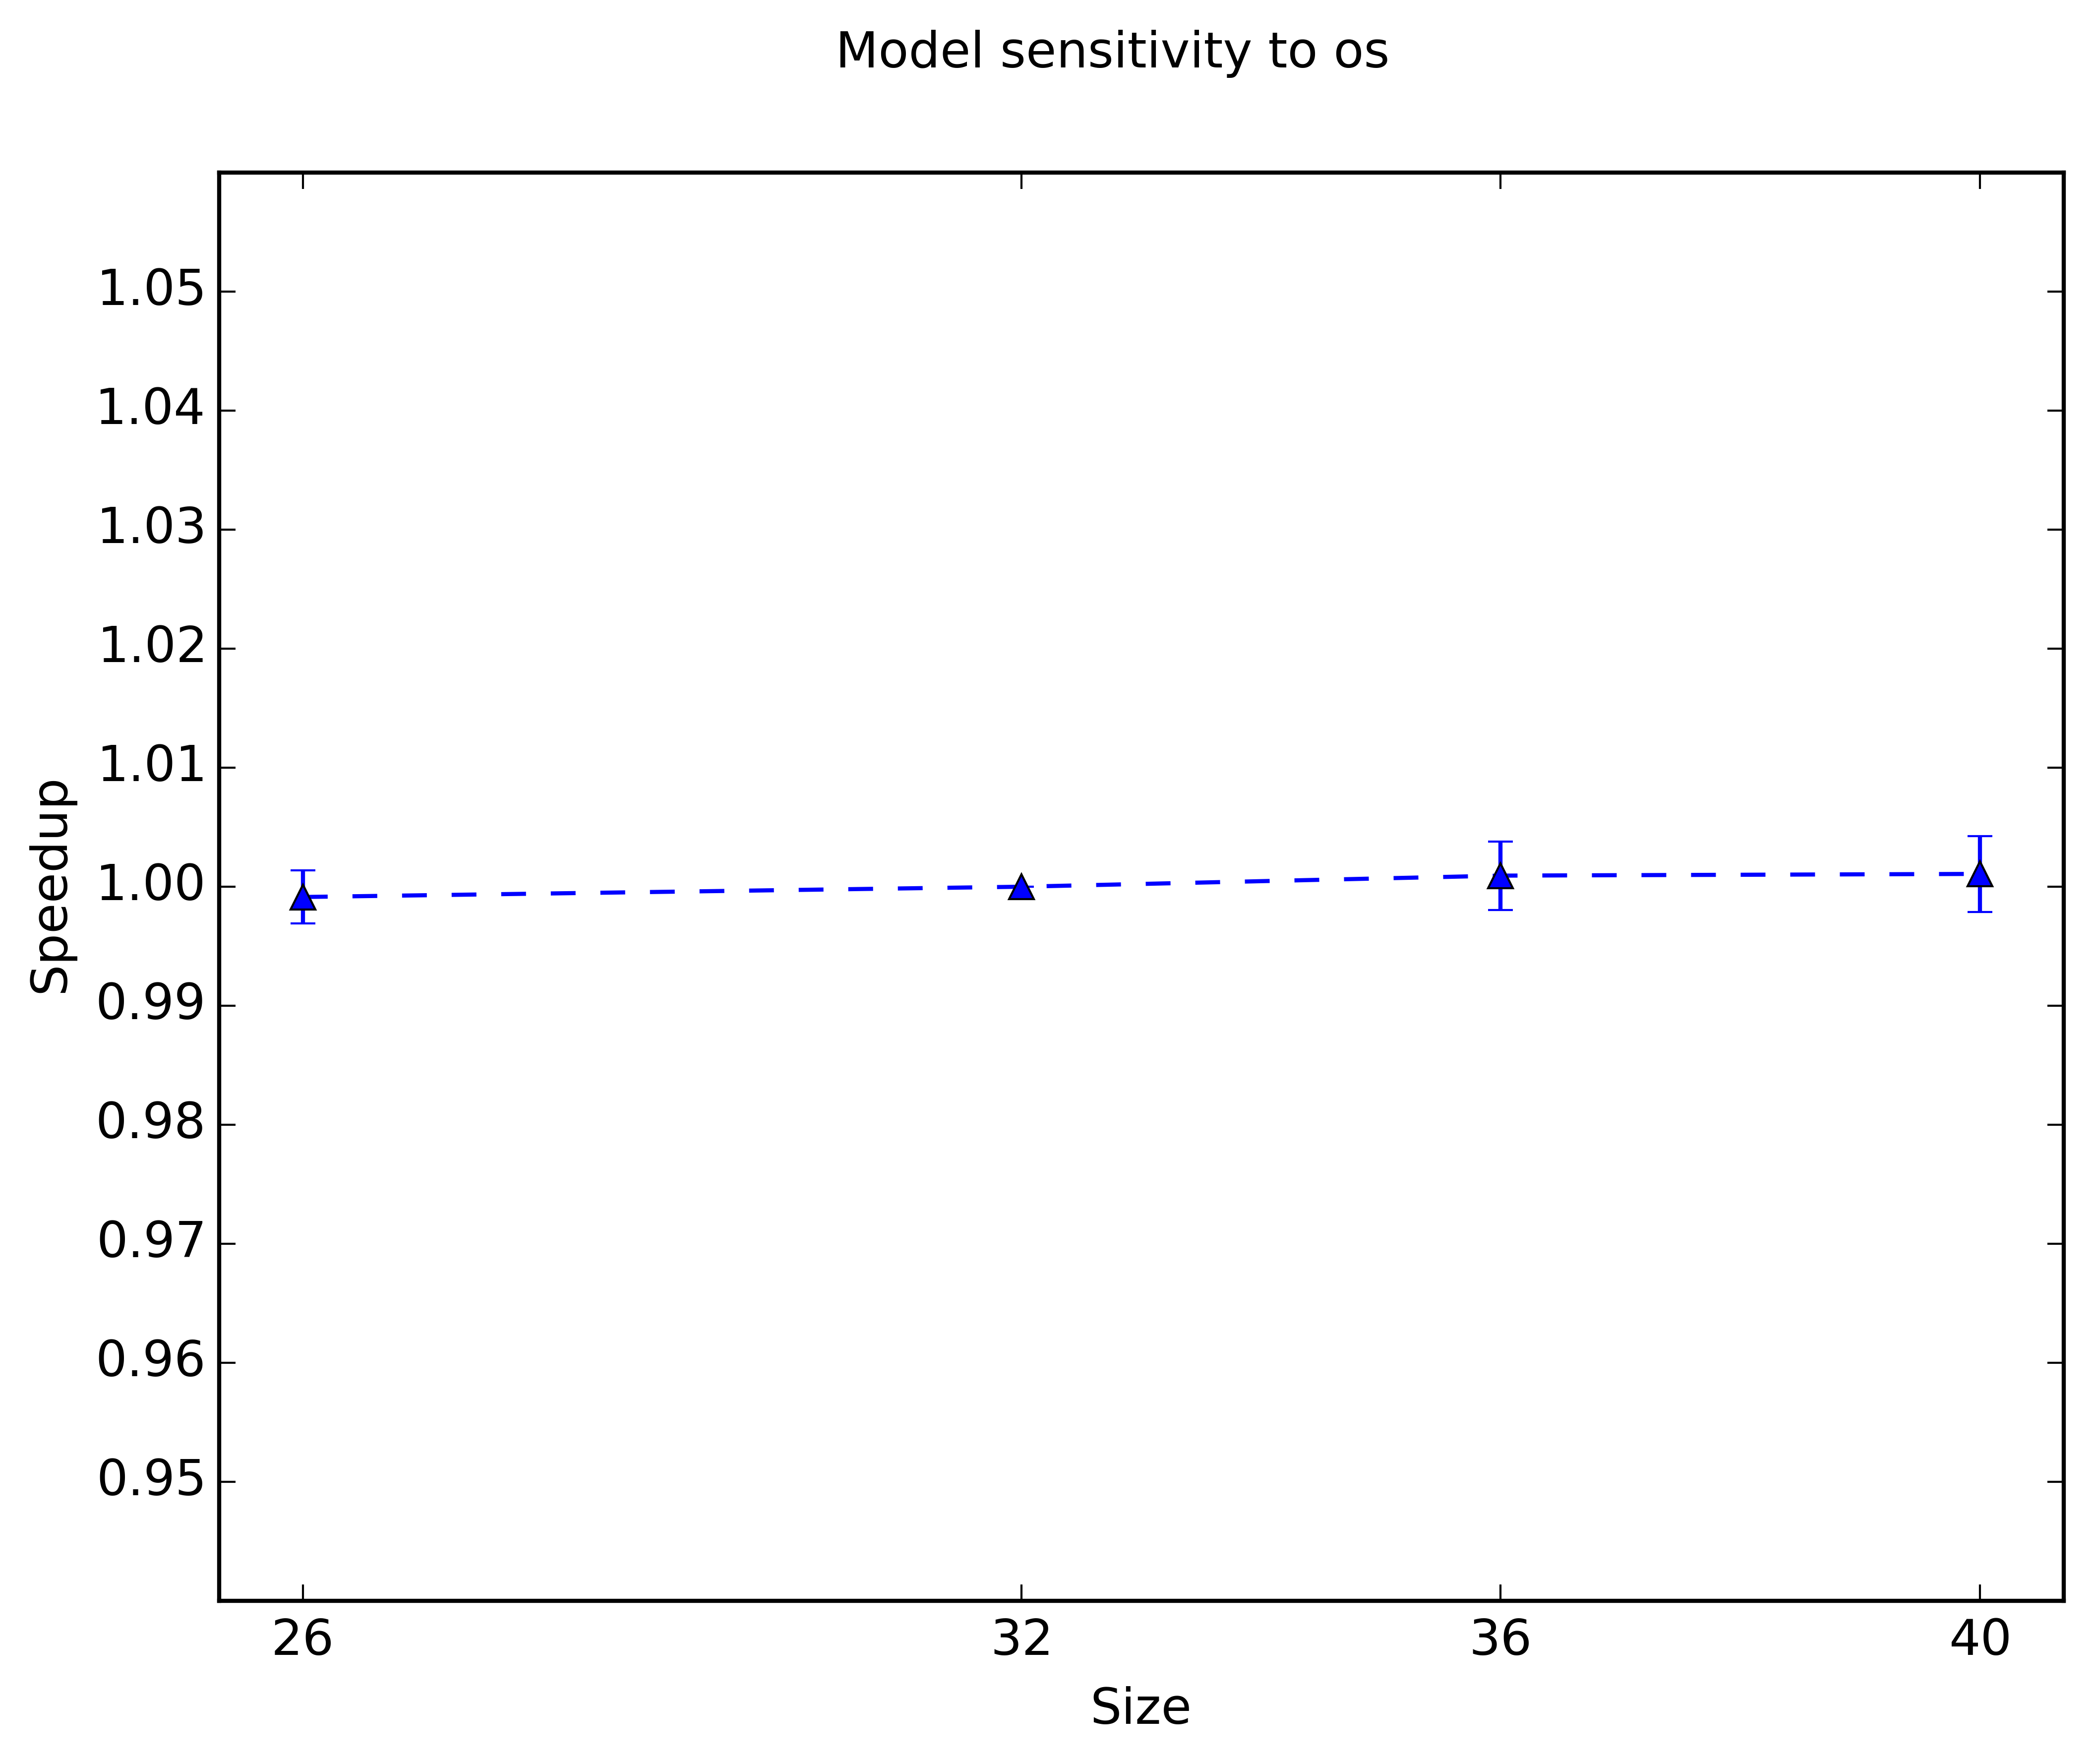
\includegraphics[width=\textwidth]{figures/processor_model/os}
                \label{fig:processor_model:sensitivity:os}
        \end{subfigure}
        \begin{subfigure}[b]{0.5\textwidth}
                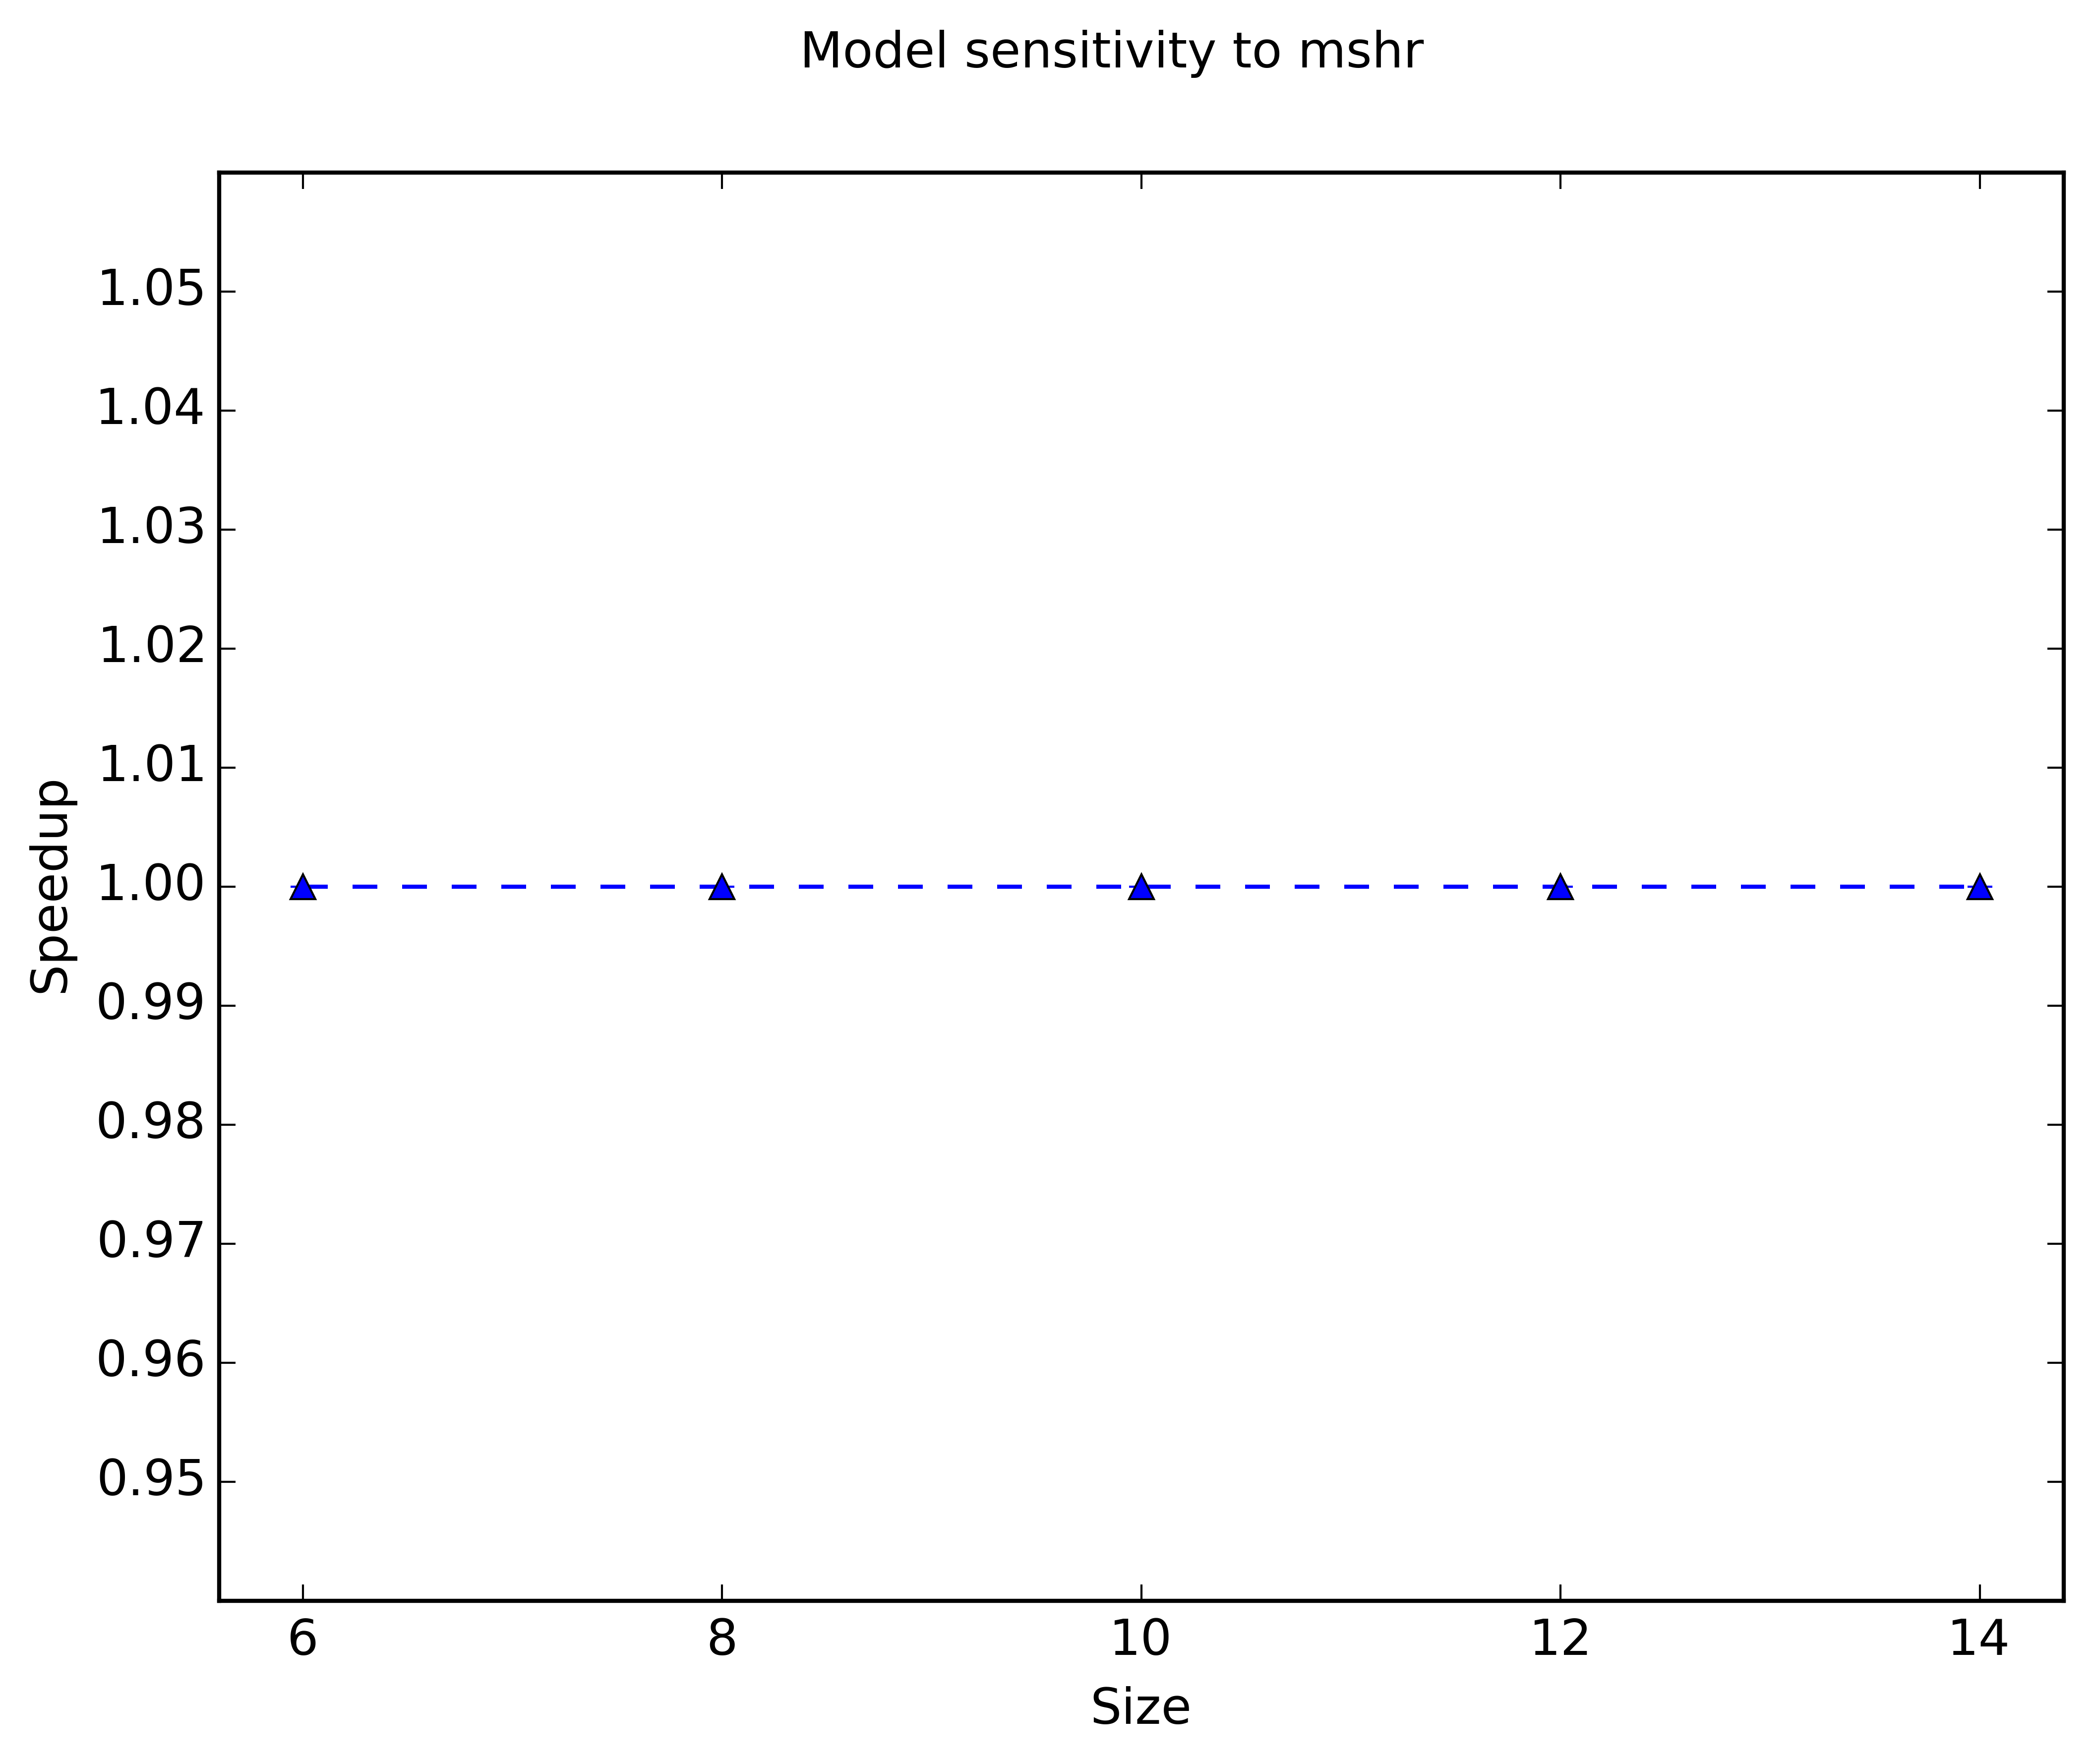
\includegraphics[width=\textwidth]{figures/processor_model/mshr}
                \label{fig:processor_model:sensitivity:mshr}
        \end{subfigure}%
        \begin{subfigure}[b]{0.5\textwidth}
                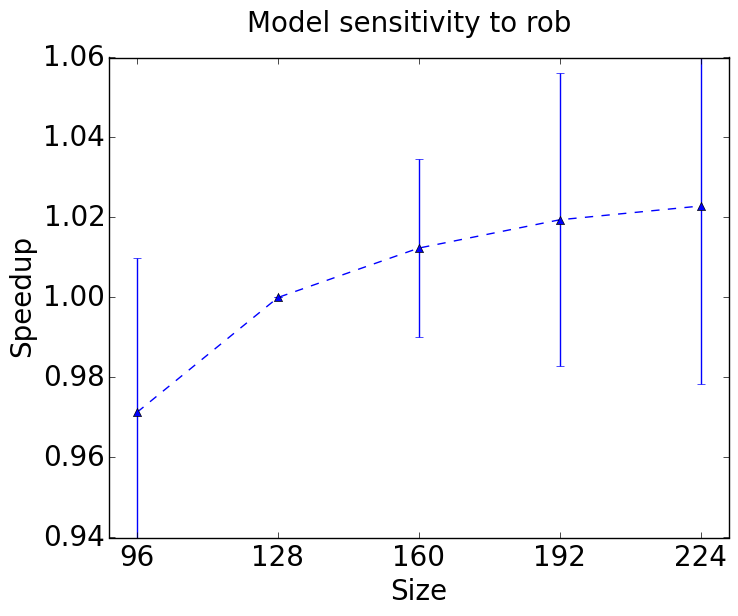
\includegraphics[width=\textwidth]{figures/processor_model/rob}
                \label{fig:processor_model:sensitivity:rob}
        \end{subfigure}
        \begin{subfigure}[b]{0.5\textwidth}
                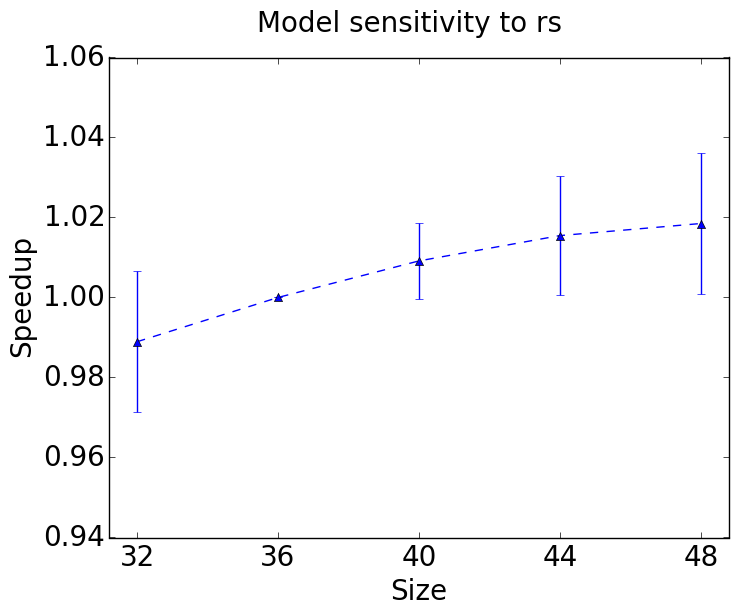
\includegraphics[width=\textwidth]{figures/processor_model/rs}
                \label{fig:processor_model:sensitivity:rs}
        \end{subfigure}%
        \caption{Core model property sensitivity}\label{fig:processor_model:sensitivity}
\end{figure}

Figure~\ref{fig:processor_model:sensitivity} shows the average speedup of all benchmarks when we vary our five selected properties; Outstanding loads (ol), outstanding stores (os), L1 miss status hold registers (MSHR), re-order buffer size (rob) and reservation station entries (rs).
Outstanding loads and stores specify the number of outstanding memory requests the core can manage before it as to block at new requests.
The number of L1 MSHRs decide how many outstanding cache misses the cache can handle before it has to block on a new miss.
The size of the rob and rs together decide how many instructions can be live during execution.  
Increasing the number of live instructions can increase the amount of instruction-level parallelism (ILP) the processor can extract from the program while possibly increasing the cost of a branch miss prediction.

For all memory related properties; os, ol and mshr, we observe no improvement nor decrease in performance when varying their value.
When Increasing the size of the rob and the number of rs entries, we do observe a slight increase in performance.
The numbers show an average performance increase of about 2\% with more rob entries, and about a 3\% increase with more rs entries.
We also observe that these increases come at the cost of a respectively 75\% and 50\% storage increase.
In addition, we observe that the standard deviation in both cases is about the same as the average performance increase.
When reviewed, these facts lead us to conclude that the processor model we have presented based on the Nehalem architecture is stable and that we have no obvious performance gains from small adjustments.
As a result, we decide to continue use of this model for the rest of our experiments without making any adjustments.

Considering that we base our model properties on an actual architecture and that our simulator strives to simulate the core model of that same architecture, it is not a far-fetched result observing little sensitivity to property changes.
During the design process of the architecture, it is natural to expect that the designers made a conscious choice between speed and area using a similar analysis.
The final properties would then most likely have been selected to provide a stable middle ground, which we see reflected in our simulation results.